\chapter{Risks and Saftey}
\label{sec: Risk_and_saftey}
\vspace{-3mm}
\section{Project Identification Risks}
\subsection{Safety}
    This project deals with fast-spinning props and live electricity. Caution must be taken when the prototype is switched on and whenever the wires are being handheld. To minimize this risk, when working with the proof of concept the power source should be disconnected, this will prevent accidental activations as well as electrocution.
    \vspace{-1mm}
    \subsection{Technical Risks}
    These risks pertain to the risk of equipment or component failure. If equipment malfunction or component failure occurs this could cause harm to either the user or the prototype. To minimize this risk, thorough testing of the equipment and components should be done to ensure they are operating how to be expected. Another potential technical risk is whether the thrust and control system would be able to be operated with enough accuracy and speed to allow for directional thrust. This risk can be reduced through the proper design of the system and the correct selection of components. 
    \vspace{-1mm}
    \subsection{Financial Risks}
    Financial risks include going over budget or standing more than expected. This risk can be minimized through proper budget planning to ensure an accurate budget has been created. Minimizing the technical risk, as mentioned previously, will prevent components or equipment from needing to be replaced.
% \subsection{Scheduling risk}
%     There is a limited amount of time to complete this project and as such there is a very tight schedule. Unexpected delays could have catastrophic effects on the project and could potentially cause it to become incomplete. To prevent this from occurring, a detailed plan should be devised, and the student should follow it as closely as possible.  
% \subsection{Resources risk}
%     This risk relates closely to the previous risk, scheduling risk, as a delay in resources can cause a delay in the entire project. Ordering components or sending designs to be created at the workshop should be done in far enough advance such that if there are any unexpected delays, it will not crucially affect the project's schedule. It can also be reduced by choosing components that are readily available and easy to obtain.\\
\vspace{-5mm}
\section{Lab Safety Reports}
    Below are two summarized safety report for the Mechatronics and Structures lab. The full safety reports can be found on the project folder.

            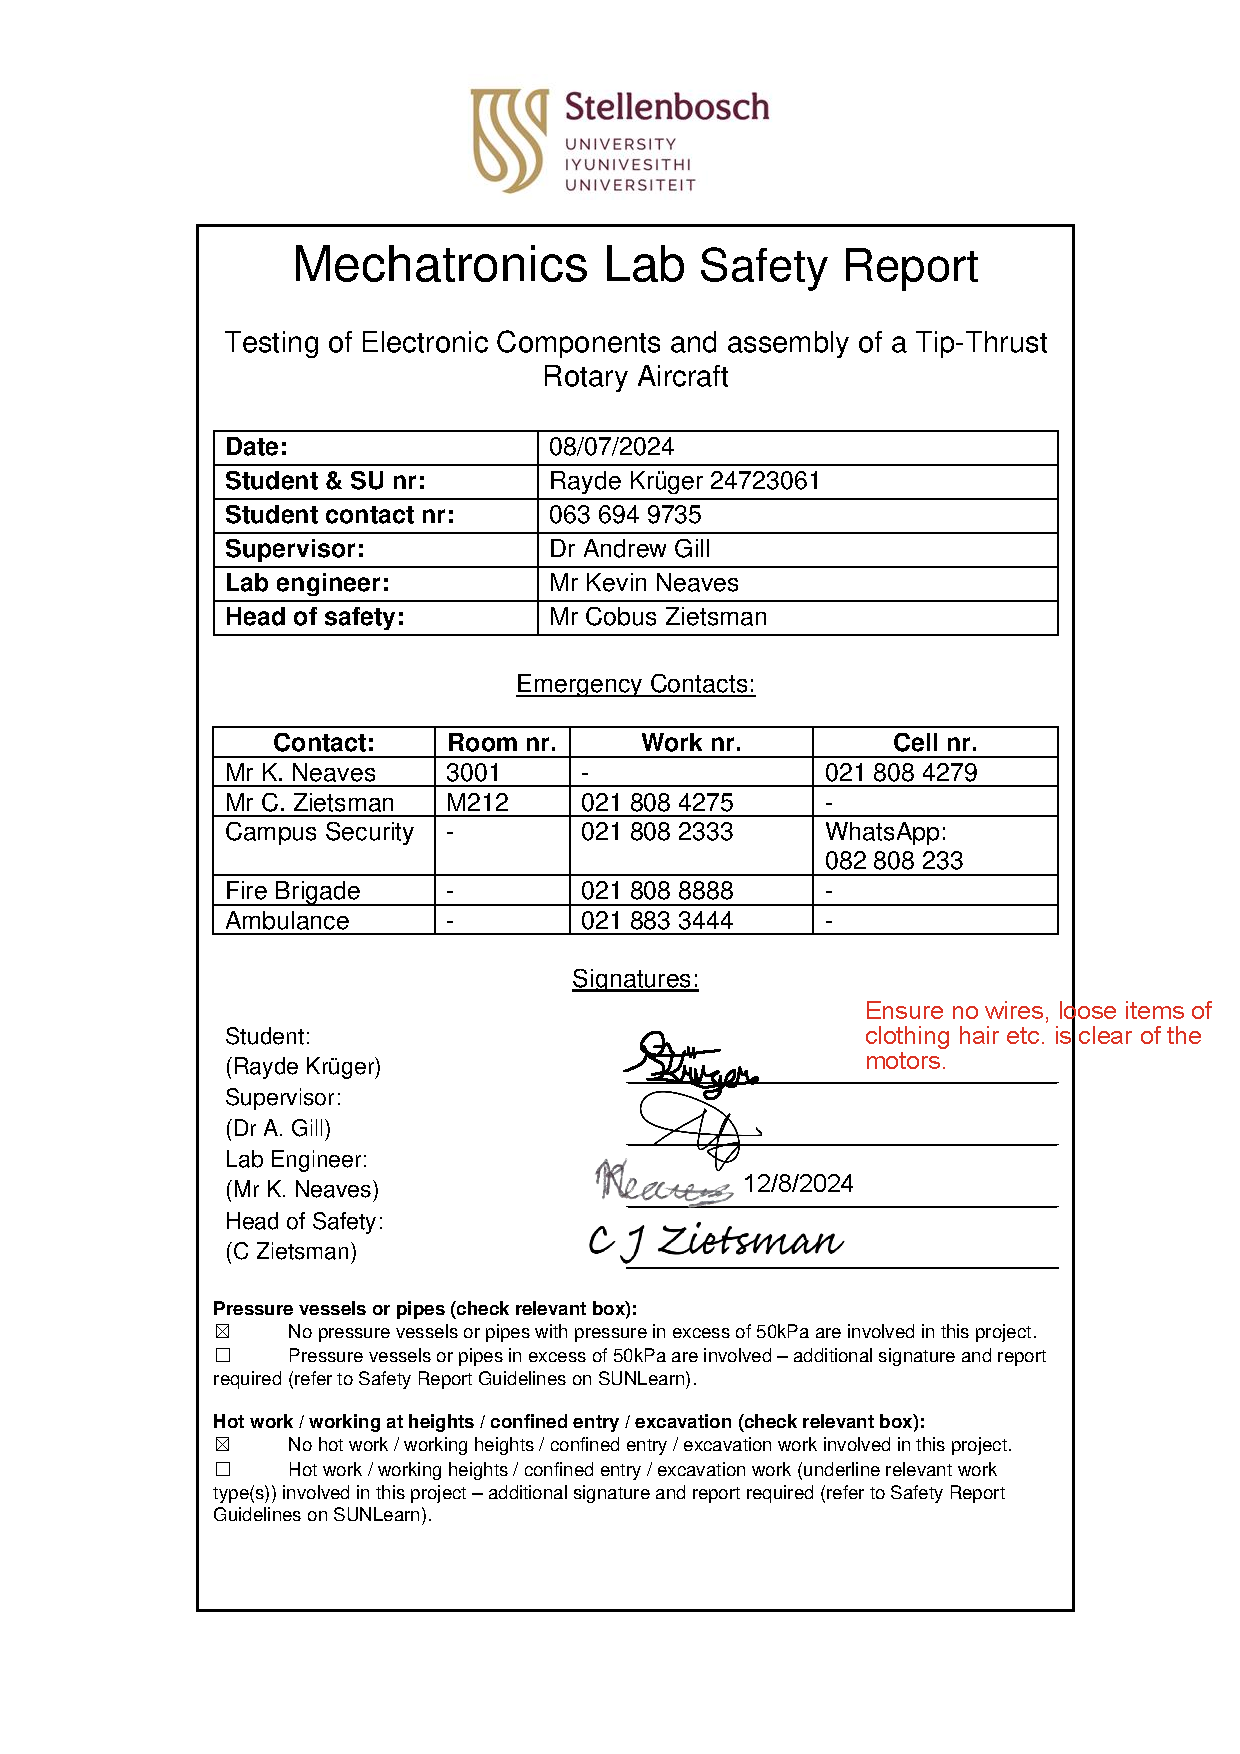
\includepdf[pages=1]{Appendix Documents/Mechatronics Lab Saftey Report_ Zietsman signed.pdf}
            \subsection*{Experimental Procedure}
            \vspace*{-1mm}
                \begin{itemize}
                    \item \textbf{Electronics testing set up}:
                        The details of the datasheet for each component should be known as well as the location of the emergency stop button before testing the components can begin. All wires should be labeled and undamaged. The connections as well as the power supply and oscilloscope should be checked.
                        \vspace*{-1mm}
                    \item \textbf{Testing procedure for electronics}:
                        Once all the circuit has been connected according to the wiring diagram and the microcontroller is outputting the correct signal, the power supply can be switched on. The test program can be run to observe the system's behavior. 
                        \vspace*{-1mm}
                    \item \textbf{Assembly for tip-thrust rotary aircraft}:
                        Before assembling ensure that all components are operating correctly and are undamaged. Assemble the aircraft as described by the CAD model and install the electronics according to the datasheets, ensuring all connections are secure. 
                        \vspace*{-1mm}
                    \item \textbf{Shut down procedure}:
                        Stop the program on the microcontroller then turn off the power supply and oscilloscope. Disassemble and store the components in the storage locker. Clean up the workstation before leaving.
                \end{itemize}

                \small
                \vspace*{-3mm}
                \begin{longtable}{|llllc|}
                \caption{Mechatronics lab risk table}\\
                \hline
                \rowcolor[HTML]{D1D1D1} 
                \multicolumn{1}{|c|}{\cellcolor[HTML]{D1D1D1}Activity}                                                                & \multicolumn{1}{c|}{\cellcolor[HTML]{D1D1D1}Risk}                                                         & \multicolumn{1}{c|}{\cellcolor[HTML]{D1D1D1}\begin{tabular}[c]{@{}c@{}}Risk   \\ Type* \\ (P/E)\end{tabular}} & \multicolumn{1}{c|}{\cellcolor[HTML]{D1D1D1}\begin{tabular}[c]{@{}c@{}}Mitigating\\ Steps\end{tabular}}                                                    & \begin{tabular}[c]{@{}c@{}}Classification \\ of Risk \\ Severity\end{tabular} \\ \hline
                \rowcolor[HTML]{D1D1D1} 
                \multicolumn{5}{|c|}{\cellcolor[HTML]{D1D1D1}GENERAL}                                                                                                                                                                                                                                                                                                                                                                                                                                                                                                                                          \\ \hline
                \multicolumn{1}{|l|}{\begin{tabular}[c]{@{}l@{}}Moving\\ around\\ the lab\end{tabular}}                               & \multicolumn{1}{l|}{\begin{tabular}[c]{@{}l@{}}Tripping or\\ knocking over\\ equipment\end{tabular}}      & \multicolumn{1}{l|}{P}                                                                                        & \multicolumn{1}{l|}{\begin{tabular}[c]{@{}l@{}}Be aware of the \\ surrounding equipment\\  and environment when \\ walking in the lab\end{tabular}}        & \begin{tabular}[c]{@{}c@{}}Acceptable   \\ risk\end{tabular}                  \\ \hline
                \multicolumn{1}{|l|}{\begin{tabular}[c]{@{}l@{}}Power\\ outages\end{tabular}}                                         & \multicolumn{1}{l|}{\begin{tabular}[c]{@{}l@{}}Data   loss and \\ damage to \\ equipment\end{tabular}}    & \multicolumn{1}{l|}{E}                                                                                        & \multicolumn{1}{l|}{\begin{tabular}[c]{@{}l@{}}Check   the loadshedding \\ schedule beforehand\end{tabular}}                                               & \begin{tabular}[c]{@{}c@{}}Possible \\   risk\end{tabular}                    \\ \hline
                \multicolumn{1}{|l|}{\begin{tabular}[c]{@{}l@{}}Personal\\ items\end{tabular}}                                        & \multicolumn{1}{l|}{Theft of   items}                                                                     & \multicolumn{1}{l|}{P}                                                                                        & \multicolumn{1}{l|}{\begin{tabular}[c]{@{}l@{}}Don’t   leave personal \\ items unattended\end{tabular}}                                                    & \begin{tabular}[c]{@{}c@{}}Acceptable  \\ risk\end{tabular}                   \\ \hline
                \rowcolor[HTML]{D1D1D1} 
                \multicolumn{5}{|c|}{\cellcolor[HTML]{D1D1D1}TESTING PHASE}                                                                                                                                                                                                                                                                                                                                                                                                                                                                                                                                    \\ \hline
                \multicolumn{1}{|l|}{\multirow{-3}{*}{\begin{tabular}[c]{@{}l@{}}Installing\\ electrical \\ components\end{tabular}}} & \multicolumn{1}{l|}{Electric   shocks}                                                                    & \multicolumn{1}{l|}{P}                                                                                        & \multicolumn{1}{l|}{\begin{tabular}[c]{@{}l@{}}Ensure   the power is off \\ when working with the \\ components\end{tabular}}                              & \begin{tabular}[c]{@{}c@{}}Possible   \\ risk\end{tabular}                    \\ \cline{2-5} 
                \multicolumn{1}{|l|}{}                                                                                                & \multicolumn{1}{l|}{\begin{tabular}[c]{@{}l@{}}Shorting \\ electrical \\ components\end{tabular}}          & \multicolumn{1}{l|}{E}                                                                                        & \multicolumn{1}{l|}{\begin{tabular}[c]{@{}l@{}}Ensure   all components \\ are connected correctly \\ before powering them\end{tabular}}                    & \begin{tabular}[c]{@{}c@{}}Acceptable   \\ risk\end{tabular}                  \\ \cline{2-5} 
                \multicolumn{1}{|l|}{}                                                                                                & \multicolumn{1}{l|}{\begin{tabular}[c]{@{}l@{}}Incorrect   \\ connections\end{tabular}}                   & \multicolumn{1}{l|}{E}                                                                                        & \multicolumn{1}{l|}{\begin{tabular}[c]{@{}l@{}}Ensure   components are \\ connected according to \\ the wiring diagram\end{tabular}}                       & \begin{tabular}[c]{@{}c@{}}Acceptable   \\ risk\end{tabular}                  \\ \hline
                \multicolumn{1}{|l|}{\begin{tabular}[c]{@{}l@{}}Using hand\\ tools\end{tabular}}                                      & \multicolumn{1}{l|}{\begin{tabular}[c]{@{}l@{}}Injuries   due to\\ slippage\end{tabular}}                 & \multicolumn{1}{l|}{P}                                                                                        & \multicolumn{1}{l|}{\begin{tabular}[c]{@{}l@{}}Ensure   if a tool slips,\\  no injuries can occur\end{tabular}}                                            & \begin{tabular}[c]{@{}c@{}}Acceptable   \\ risk\end{tabular}                  \\ \hline
                \multicolumn{1}{|l|}{\begin{tabular}[c]{@{}l@{}}Installing\\ motors\end{tabular}}                                     & \multicolumn{1}{l|}{\begin{tabular}[c]{@{}l@{}}Dropping \\ motors\end{tabular}}                           & \multicolumn{1}{l|}{E}                                                                                        & \multicolumn{1}{l|}{\begin{tabular}[c]{@{}l@{}}Handle   motors \\ with care\end{tabular}}                                                                  & \begin{tabular}[c]{@{}c@{}}Acceptable   \\ risk\end{tabular}                  \\ \hline
                \multicolumn{1}{|l|}{\begin{tabular}[c]{@{}l@{}}Assembling\\ rotor\end{tabular}}                                      & \multicolumn{1}{l|}{\begin{tabular}[c]{@{}l@{}}Pinching \\ fingers\end{tabular}}                          & \multicolumn{1}{l|}{P}                                                                                        & \multicolumn{1}{l|}{\begin{tabular}[c]{@{}l@{}}Ensure   fingers are not\\ caught in between \\ components while \\ assembling\end{tabular}}                & \begin{tabular}[c]{@{}c@{}}Acceptable   \\ risk\end{tabular}                  \\ \hline
                \multicolumn{1}{|l|}{\begin{tabular}[c]{@{}l@{}}Incorrect\\ Calibration\end{tabular}}                                 & \multicolumn{1}{l|}{\begin{tabular}[c]{@{}l@{}}Aircraft   \\ is uncontrollable\end{tabular}}              & \multicolumn{1}{l|}{P/E}                                                                                      & \multicolumn{1}{l|}{\begin{tabular}[c]{@{}l@{}}After   calibrating the \\ pitch, ensure the \\ readings are correct\end{tabular}}                          & \begin{tabular}[c]{@{}c@{}}Acceptable   \\ risk\end{tabular}                  \\ \hline
                \multicolumn{1}{|l|}{\begin{tabular}[c]{@{}l@{}}Loose wires \\ or clothing \\ caught in the \\ motors\end{tabular}}   & \multicolumn{1}{l|}{\begin{tabular}[c]{@{}l@{}}Getting   items \\ entangled by\\ the motors\end{tabular}} & \multicolumn{1}{l|}{P/E}                                                                                      & \multicolumn{1}{l|}{\begin{tabular}[c]{@{}l@{}}Don’t   wear loose \\ clothing and ensure \\ any loose items are \\ kept away from the motors\end{tabular}} & \begin{tabular}[c]{@{}c@{}}Acceptable   \\ risk\end{tabular}                  \\ \hline
                \multicolumn{1}{|l|}{}                                                                                                & \multicolumn{1}{l|}{\begin{tabular}[c]{@{}l@{}}Impact   with\\  the rotor\end{tabular}}                   & \multicolumn{1}{l|}{P/E}                                                                                      & \multicolumn{1}{l|}{\begin{tabular}[c]{@{}l@{}}Ensure   there are no \\ obstructions with the \\ rotors’ path\end{tabular}}                                & \begin{tabular}[c]{@{}c@{}}Possible   \\ risk\end{tabular}                    \\ \cline{2-5} 
                \multicolumn{1}{|l|}{\multirow{-2}{*}{\begin{tabular}[c]{@{}l@{}}Rotor\\ turning\end{tabular}}}                       & \multicolumn{1}{l|}{\begin{tabular}[c]{@{}l@{}}Items   detach \\ from the rotor\end{tabular}}             & \multicolumn{1}{l|}{P/E}                                                                                      & \multicolumn{1}{l|}{\begin{tabular}[c]{@{}l@{}}Check   that all items\\ are securely attached \\ to the rotor and hub\end{tabular}}                        & \begin{tabular}[c]{@{}c@{}}Possible   \\ risk\end{tabular}                    \\ \hline
                \multicolumn{1}{|l|}{\begin{tabular}[c]{@{}l@{}}Rotor   \\ turning\end{tabular}}                                      & \multicolumn{1}{l|}{\begin{tabular}[c]{@{}l@{}}Rotary   aircraft \\ tips over\end{tabular}}               & \multicolumn{1}{l|}{P/E}                                                                                      & \multicolumn{1}{l|}{\begin{tabular}[c]{@{}l@{}}Ensure   the base\\ is firmly secured\end{tabular}}                                                         & \begin{tabular}[c]{@{}c@{}}Possible   \\ risk\end{tabular}                    \\ \hline
                \multicolumn{1}{|l|}{\begin{tabular}[c]{@{}l@{}}Load cell \\ failure\end{tabular}}                                    & \multicolumn{1}{l|}{\begin{tabular}[c]{@{}l@{}}Incorrect\\ readings from\\ the load cells\end{tabular}}  & \multicolumn{1}{l|}{E}                                                                                        & \multicolumn{1}{l|}{\begin{tabular}[c]{@{}l@{}}Calibrate   the \\ load cells before\\ use\end{tabular}}                                                    & \begin{tabular}[c]{@{}c@{}}Acceptable   \\ risk\end{tabular}                  \\ \hline
                \multicolumn{1}{|l|}{\multirow{-2}{*}{\begin{tabular}[c]{@{}l@{}}Testing  \\ motor\end{tabular}}}                     & \multicolumn{1}{l|}{\begin{tabular}[c]{@{}l@{}}Motors   \\ overheat\end{tabular}}                         & \multicolumn{1}{l|}{E}                                                                                        & \multicolumn{1}{l|}{\begin{tabular}[c]{@{}l@{}}Ensure   the motors \\ operate within the \\ rated values\end{tabular}}                                     & \begin{tabular}[c]{@{}c@{}}Acceptable   \\ risk\end{tabular}                  \\ \cline{2-5} 
                \multicolumn{1}{|l|}{}                                                                                                & \multicolumn{1}{l|}{\begin{tabular}[c]{@{}l@{}}Burns   occur \\ from motor \\ overheating\end{tabular}}   & \multicolumn{1}{l|}{P}                                                                                        & \multicolumn{1}{l|}{\begin{tabular}[c]{@{}l@{}}Ensure   the motors\\ operate within the \\ rated values\end{tabular}}                                      & \begin{tabular}[c]{@{}c@{}}Acceptable   \\ risk\end{tabular}                  \\ \hline
                \multicolumn{1}{|l|}{\begin{tabular}[c]{@{}l@{}}Testing   \\ software\end{tabular}}                                   & \multicolumn{1}{l|}{\begin{tabular}[c]{@{}l@{}}Code not   \\ working as\\ intended\end{tabular}}          & \multicolumn{1}{l|}{P/E}                                                                                      & \multicolumn{1}{l|}{\begin{tabular}[c]{@{}l@{}}Ensure   the code \\ is fully understood\\  before it is uploaded\end{tabular}}                             & \begin{tabular}[c]{@{}c@{}}Acceptable   \\ risk\end{tabular}                  \\ \hline
                \multicolumn{1}{|l|}{\begin{tabular}[c]{@{}l@{}}Backing   \\ up data\end{tabular}}                                    & \multicolumn{1}{l|}{Data   loss}                                                                          & \multicolumn{1}{l|}{E}                                                                                        & \multicolumn{1}{l|}{\begin{tabular}[c]{@{}l@{}}Use a   USB/ hard\\ drive which is frequently \\ updated.\end{tabular}}                                     & \begin{tabular}[c]{@{}c@{}}Acceptable   \\ risk\end{tabular}                  \\ \hline
                \end{longtable}


\includepdf[pages=1     ]{Appendix Documents/Structure's Lab Saftey Report-Rayde Krüger-24723061_Zietsman_Signed.pdf}
    \subsection*{Experimental Procedure}
        Please see Section~\ref{sec: Experiment} to see the full experimental procedure for the locked rotor and dynamic tests.
    \small
    \begin{longtable}{|llllc|}
    \hline
    \rowcolor[HTML]{D0CECE} 
    \multicolumn{1}{|c|}{\cellcolor[HTML]{D0CECE}Activity}                                                                   & \multicolumn{1}{c|}{\cellcolor[HTML]{D0CECE}Risk}                                                        & \multicolumn{1}{c|}{\cellcolor[HTML]{D0CECE}\begin{tabular}[c]{@{}c@{}}Risk   \\ Type* \\ (P/E)\end{tabular}} & \multicolumn{1}{c|}{\cellcolor[HTML]{D0CECE}\begin{tabular}[c]{@{}c@{}}Mitigating   \\ Steps\end{tabular}}                                                 & \begin{tabular}[c]{@{}c@{}}Classification \\   of Risk\\ Severity\end{tabular} \\ \hline
    \rowcolor[HTML]{D0CECE} 
    \multicolumn{5}{|c|}{\cellcolor[HTML]{D0CECE}GENERAL}                                                                                                                                                                                                                                                                                                                                                                                                                                                                                                                                             \\ \hline
    \multicolumn{1}{|l|}{\begin{tabular}[c]{@{}l@{}}Moving around \\ the lab\end{tabular}}                                   & \multicolumn{1}{l|}{\begin{tabular}[c]{@{}l@{}}Tripping   or \\ knocking over\\ equipment\end{tabular}}  & \multicolumn{1}{l|}{P}                                                                                        & \multicolumn{1}{l|}{\begin{tabular}[c]{@{}l@{}}Be aware of the \\ surrounding equipment \\ and environment when \\ walking in the lab\end{tabular}}        & \begin{tabular}[c]{@{}c@{}}Acceptable \\  risk\end{tabular}                    \\ \hline
    \multicolumn{1}{|l|}{\begin{tabular}[c]{@{}l@{}}Power   \\ outages\end{tabular}}                                         & \multicolumn{1}{l|}{\begin{tabular}[c]{@{}l@{}}Data   loss \\ and damage \\ to equipment\end{tabular}}   & \multicolumn{1}{l|}{E}                                                                                        & \multicolumn{1}{l|}{\begin{tabular}[c]{@{}l@{}}Check   the loadshedding\\ schedule beforehand\end{tabular}}                                                & \begin{tabular}[c]{@{}c@{}}Possible   \\ risk\end{tabular}                     \\ \hline
    \multicolumn{1}{|l|}{\begin{tabular}[c]{@{}l@{}}Personal   \\ items\end{tabular}}                                        & \multicolumn{1}{l|}{\begin{tabular}[c]{@{}l@{}}Theft of   \\ items\end{tabular}}                         & \multicolumn{1}{l|}{P}                                                                                        & \multicolumn{1}{l|}{\begin{tabular}[c]{@{}l@{}}Don’t   leave personal\\  items unattended\end{tabular}}                                                    & \begin{tabular}[c]{@{}c@{}}Acceptable   \\ risk\end{tabular}                   \\ \hline
    \rowcolor[HTML]{D0CECE} 
    \multicolumn{5}{|c|}{\cellcolor[HTML]{D0CECE}TESTING PHASE}                                                                                                                                                                                                                                                                                                                                                                                                                                                                                                                                       \\ \hline
    \multicolumn{1}{|l|}{}                                                                                                   & \multicolumn{1}{l|}{\begin{tabular}[c]{@{}l@{}}Electric   \\ shocks\end{tabular}}                        & \multicolumn{1}{l|}{P}                                                                                        & \multicolumn{1}{l|}{\begin{tabular}[c]{@{}l@{}}Ensure   the power is \\ off when working \\ with the components\end{tabular}}                              & \begin{tabular}[c]{@{}c@{}}Possible   \\ risk\end{tabular}                     \\ \cline{2-5} 
    \multicolumn{1}{|l|}{}                                                                                                   & \multicolumn{1}{l|}{\begin{tabular}[c]{@{}l@{}}Shorting   \\ electrical \\ components\end{tabular}}      & \multicolumn{1}{l|}{E}                                                                                        & \multicolumn{1}{l|}{\begin{tabular}[c]{@{}l@{}}Ensure   all components\\ are connected correctly \\ before powering them\end{tabular}}                     & \begin{tabular}[c]{@{}c@{}}Acceptable  \\ risk\end{tabular}                    \\ \cline{2-5} 
    \multicolumn{1}{|l|}{\multirow{-3}{*}{\begin{tabular}[c]{@{}l@{}}Installing   \\ electrical \\ components\end{tabular}}} & \multicolumn{1}{l|}{\begin{tabular}[c]{@{}l@{}}Incorrect   \\ connections\end{tabular}}                  & \multicolumn{1}{l|}{E}                                                                                        & \multicolumn{1}{l|}{\begin{tabular}[c]{@{}l@{}}Ensure components are \\ connected according to\\  the wiring diagram\end{tabular}}                         & \begin{tabular}[c]{@{}c@{}}Acceptable   \\ risk\end{tabular}                   \\ \hline
    \multicolumn{1}{|l|}{\begin{tabular}[c]{@{}l@{}}Using   \\ hand tools\end{tabular}}                                      & \multicolumn{1}{l|}{\begin{tabular}[c]{@{}l@{}}Injuries   \\ due to \\ slippage\end{tabular}}            & \multicolumn{1}{l|}{P}                                                                                        & \multicolumn{1}{l|}{\begin{tabular}[c]{@{}l@{}}Ensure if a tool slips, \\ no injuries can occur\end{tabular}}                                              & \begin{tabular}[c]{@{}c@{}}Acceptable   \\ risk\end{tabular}                   \\ \hline
    \multicolumn{1}{|l|}{\begin{tabular}[c]{@{}l@{}}Installing   \\ motors\end{tabular}}                                     & \multicolumn{1}{l|}{\begin{tabular}[c]{@{}l@{}}Dropping   \\ motors\end{tabular}}                        & \multicolumn{1}{l|}{E}                                                                                        & \multicolumn{1}{l|}{\begin{tabular}[c]{@{}l@{}}Handle   motors \\ with care\end{tabular}}                                                                  & \begin{tabular}[c]{@{}c@{}}Acceptable  \\  risk\end{tabular}                   \\ \hline
    \multicolumn{1}{|l|}{\begin{tabular}[c]{@{}l@{}}Assembling  \\ rotor\end{tabular}}                                       & \multicolumn{1}{l|}{\begin{tabular}[c]{@{}l@{}}Pinching   \\ fingers\end{tabular}}                       & \multicolumn{1}{l|}{P}                                                                                        & \multicolumn{1}{l|}{\begin{tabular}[c]{@{}l@{}}Ensure   fingers are\\ not caught in\\ between components\\ while assembling\end{tabular}}                  & \begin{tabular}[c]{@{}c@{}}Acceptable \\  risk\end{tabular}                    \\ \hline
    \multicolumn{1}{|l|}{\begin{tabular}[c]{@{}l@{}}Incorrect  \\ Calibration\end{tabular}}                                  & \multicolumn{1}{l|}{\begin{tabular}[c]{@{}l@{}}Aircraft   is\\ uncontrollable\end{tabular}}              & \multicolumn{1}{l|}{P/E}                                                                                      & \multicolumn{1}{l|}{\begin{tabular}[c]{@{}l@{}}After   calibrating the \\ pitch, ensure the \\ readings are correct\end{tabular}}                          & \begin{tabular}[c]{@{}c@{}}Acceptable  \\ risk\end{tabular}                    \\ \hline
    \multicolumn{1}{|l|}{\begin{tabular}[c]{@{}l@{}}Loose wires \\ or clothing \\ caught in the \\ motors\end{tabular}}      & \multicolumn{1}{l|}{\begin{tabular}[c]{@{}l@{}}Getting items\\  entangled by\\ the motors\end{tabular}}  & \multicolumn{1}{l|}{P/E}                                                                                      & \multicolumn{1}{l|}{\begin{tabular}[c]{@{}l@{}}Don’t   wear loose \\ clothing and ensure \\ any loose items are \\ kept away from the motors\end{tabular}} & \begin{tabular}[c]{@{}c@{}}Acceptable   \\ risk\end{tabular}                   \\ \hline
    \multicolumn{1}{|l|}{}                                                                                                   & \multicolumn{1}{l|}{\begin{tabular}[c]{@{}l@{}}Impact with \\ the rotor\end{tabular}}                    & \multicolumn{1}{l|}{P/E}                                                                                      & \multicolumn{1}{l|}{\begin{tabular}[c]{@{}l@{}}Ensure   there are \\ no obstructions\\ with the rotors’ path\end{tabular}}                                 & \begin{tabular}[c]{@{}c@{}}Possible   \\ risk\end{tabular}                     \\ \cline{2-5} 
    \multicolumn{1}{|l|}{}                                                                                                   & \multicolumn{1}{l|}{\begin{tabular}[c]{@{}l@{}}Items detach \\ from the rotor\end{tabular}}              & \multicolumn{1}{l|}{P/E}                                                                                      & \multicolumn{1}{l|}{\begin{tabular}[c]{@{}l@{}}Check   that all items \\ are securely attached\\  to the rotor and hub\end{tabular}}                       & \begin{tabular}[c]{@{}c@{}}Possible \\ risk\end{tabular}                       \\ \cline{2-5} 
    \multicolumn{1}{|l|}{\multirow{-3}{*}{\begin{tabular}[c]{@{}l@{}}Rotor   \\ turning\end{tabular}}}                       & \multicolumn{1}{l|}{\begin{tabular}[c]{@{}l@{}}Rotary aircraft \\ tips over\end{tabular}}                & \multicolumn{1}{l|}{P/E}                                                                                      & \multicolumn{1}{l|}{\begin{tabular}[c]{@{}l@{}}Ensure   the base \\ is firmly secured\end{tabular}}                                                        & \begin{tabular}[c]{@{}c@{}}Possible   \\ risk\end{tabular}                     \\ \hline
    \multicolumn{1}{|l|}{\begin{tabular}[c]{@{}l@{}}Load   cell\\  failure\end{tabular}}                                     & \multicolumn{1}{l|}{\begin{tabular}[c]{@{}l@{}}Incorrect \\ readings from\\ the load cells\end{tabular}} & \multicolumn{1}{l|}{E}                                                                                        & \multicolumn{1}{l|}{\begin{tabular}[c]{@{}l@{}}Calibrate   the load\\  cells before use\end{tabular}}                                                      & \begin{tabular}[c]{@{}c@{}}Acceptable   \\ risk\end{tabular}                   \\ \hline
    \multicolumn{1}{|l|}{}                                                                                                   & \multicolumn{1}{l|}{\begin{tabular}[c]{@{}l@{}}Motors   \\ overheat\end{tabular}}                        & \multicolumn{1}{l|}{E}                                                                                        & \multicolumn{1}{l|}{\begin{tabular}[c]{@{}l@{}}Ensure   the motors \\ operate within the \\ rated values\end{tabular}}                                     & \begin{tabular}[c]{@{}c@{}}Acceptable   \\ risk\end{tabular}                   \\ \cline{2-5} 
    \multicolumn{1}{|l|}{\multirow{-2}{*}{\begin{tabular}[c]{@{}l@{}}Testing   \\ motor\end{tabular}}}                       & \multicolumn{1}{l|}{\begin{tabular}[c]{@{}l@{}}Burns occur \\ from motor\\ overheating\end{tabular}}     & \multicolumn{1}{l|}{P}                                                                                        & \multicolumn{1}{l|}{\begin{tabular}[c]{@{}l@{}}Ensure   the motors \\ operate within the\\ rated values\end{tabular}}                                      & \begin{tabular}[c]{@{}c@{}}Acceptable \\ risk\end{tabular}                     \\ \hline
    \multicolumn{1}{|l|}{\begin{tabular}[c]{@{}l@{}}Testing  \\ software\end{tabular}}                                       & \multicolumn{1}{l|}{\begin{tabular}[c]{@{}l@{}}Code not  \\ working as\\ intended\end{tabular}}          & \multicolumn{1}{l|}{P/E}                                                                                      & \multicolumn{1}{l|}{\begin{tabular}[c]{@{}l@{}}Ensure   the code is \\ fully understood before \\ it is uploaded\end{tabular}}                             & \begin{tabular}[c]{@{}c@{}}Acceptable  \\ risk\end{tabular}                    \\ \hline
    \multicolumn{1}{|l|}{\begin{tabular}[c]{@{}l@{}}Backing   \\ up data\end{tabular}}                                       & \multicolumn{1}{l|}{Data   loss}                                                                         & \multicolumn{1}{l|}{E}                                                                                        & \multicolumn{1}{l|}{\begin{tabular}[c]{@{}l@{}}Use a   USB/ hard \\ drive which is frequently\\ updated.\end{tabular}}                                     & \begin{tabular}[c]{@{}c@{}}Acceptable  \\ risk\end{tabular}                    \\ \hline
    \end{longtable}